%!TEX root = ../thesis.tex
%*******************************************************************************
%****************************** Third Chapter **********************************
%*******************************************************************************
\chapter{Control variates, Gaia downsampling and gravitational waves}\label{ch:chapter4}

% **************************** Define Graphics Path **************************
\ifpdf
    \graphicspath{{Chapter4/Figs/Raster/}{Chapter4/Figs/PDF/}{Chapter4/Figs/}}
\else
    \graphicspath{{Chapter4/Figs/Vector/}{Chapter4/Figs/}}
\fi

\section{Gravitational waves}
Cosmological datasets are among the most data-intensive in the realms of numerical science. Thus they are a prime example of the utility of the control variate subsampling method. The particular example we shall look at to demonstrate this is an astrometric search method for individually resolvable gravitational wave sources with Gaia~\cite{Mihaylov_2020}. To introduce this, we must describe the astrometric response of stars to gravitational waves. Essentially, we can detect gravitational waves by measuring deflections of apparent star positions in the sky which correspond to gravitational waves deflecting the photons when they are emitted by the star and when they are measured at Earth. We shall examine both circumstances where the star term is included and where we can use a far-field limit that ignores the star term.

This astrometric search method was first suggested by \cite{VB}, and first derived by \cite{1996ApJ...465..566P}. Consider a metric perturbation, $h_{\mu \nu}$, due to monochromatic gravitational wave that can be written out as
%
\begin{equation}
h_{\mu \nu}(t,\textbf{x})= H_{\mu \nu} \exp( ik_{\rho}x^{\rho } )
\end{equation}
%
where $H_{\mu \nu}$ are the small complex constants satisfying transverse-traceless gauge conditions, the wavevector $k^{\mu} = (\omega, -\omega \textbf{q})$ is null, and $\textbf{q}$ is the direction unit vector of the monochromatic plane-fronted gravitational wave. Using this metric tensor one can derive the following expression for the astrometric deflection of a star as measured at Earth~\cite{Mihaylov_2020,1996ApJ...465..566P}:
%
\begin{equation}
\delta n_i = \frac{(n_i - q_i) h_{jk}(E)n^j n^k}{2(1-\textbf{q} \cdot \textbf{n})}-\frac{h_{ij}(E) n^j}{2},
\label{eq:earthterm}
\end{equation}
%
where the $n_i$ terms refer to star coordinates, and $h_{ij}(E)$ are the metric perturbations at the Earth--referred to as the ``Earth term". This expression is true at the far-field limit. Now consider a star with coordinates $(x,y,z)$, where the Earth is at the origin of this coordinate system. We label a photon emitted from this star as having spatial direction $\propto (p^x,p^y,p^z)$. Consider also a $+$ polarisation gravitational wave travelling down the $z$-axis with $A$ amplitude and $\omega$ frequency. This is without loss of generality as a simple coordinate transform could always align the $z$-axis with the gravitational wave, and the $(x,y)$ axis with the $+$ polarisation. Using \cref{eq:earthterm} this essentially translates to the apparent star positions, as observed from the Earth, being~\cite{Lasenby_2019}:
\begin{align}
    \frac{p^x}{p^z} &= \frac{x}{z}-\frac{A x \left(r z +x^2-y^2+z^2\right)\cos \left(\left(r + t \right) \omega \right) }{\omega^2 \left(r +z \right) z^2} \label{eq:px}\\
    \frac{p^y}{p^z} &= \frac{y}{z}+\frac{A y \left(r z -x^2+y^2+z^2\right)\cos \left(\left(r + t \right) \omega \right) }{\omega^2 \left(r +z \right) z^2}. \label{eq:py}
\end{align}
%
The first terms $x/z$ and $y/z$, in each of the \cref{eq:px,eq:py} respectively, are the usual direction cosines of the stars. The second terms in each are the oscillatory terms which incorporate the astrometric deflections in the apparent position of the star about the mean positions, $x/z$ and $y/z$. We can plot this projected onto a sphere in our sky, as shown in \cref{fig:epsart1}.

\begin{figure} 
\centering    
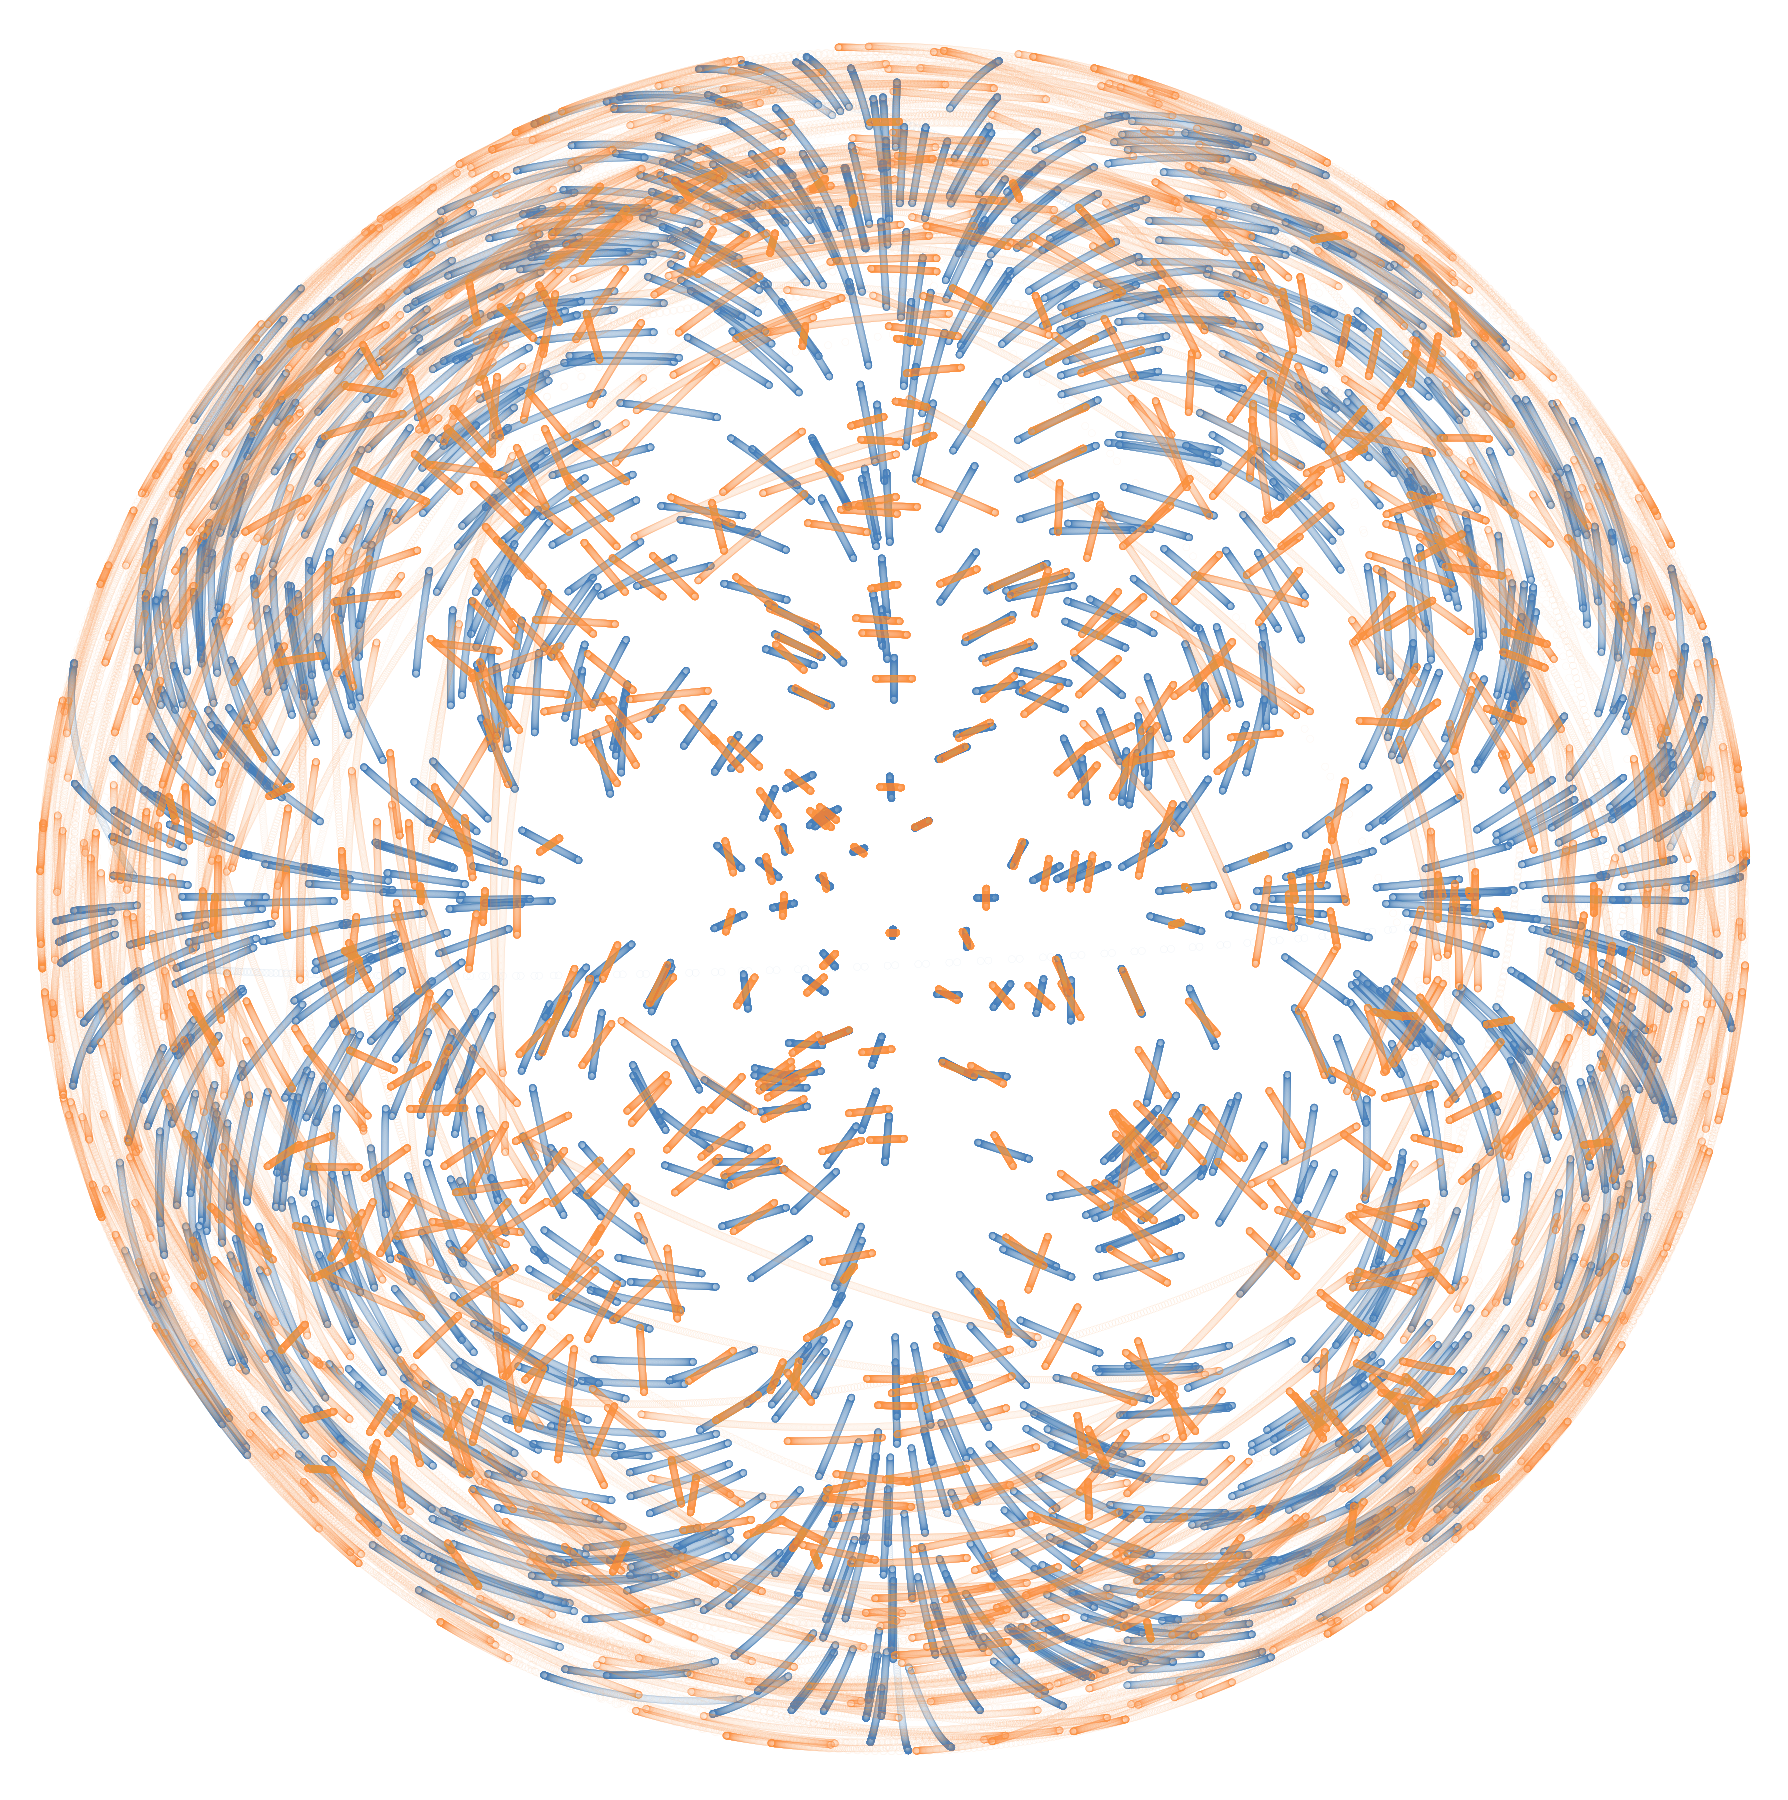
\includegraphics[width=1.0\textwidth]{Chapter4/Figs/Raster/Screenshot 2022-11-07 at 03.25.30.png}
\caption{\label{fig:epsart1} The orthographic projection of a simulated set of $1000$ stars, as observed from the Earth looking in the negative $z$ direction. With a monochromatic transverse-traceless gravitational wave travelling down the $z$-axis, the apparent positions of the stars are plotted over a whole gravitational wave time period. The blue lines represent the $+$-polarised gravitational wave results and the orange lines represent the $\times$-polarised. The 4-fold rotational symmetry of the transverse-traceless gravitational wave is clearly apparent from the rose petal pattern. We used amplitude parameter $A=0.05$. Note, the $xy$-plane is parallel with the page and orientation is such that the horizontal is the $x$-axis and vertical is $y$-axis.}
\end{figure}


\cref{fig:epsart1} is a simulation exaggerated for the purposes of demonstrating the nature of the oscillating apparent star positions that would be observed due to an incident gravitational wave's spacetime distorting effects.


\subsection{Handling of Data and Statistical Analysis for True Parameter Search}\label{sec:data_handling}

The original astrometric search analysis outlined by \cite{Mihaylov_2020} uses collected data from the Gaia satellite~\cite{2016}. Firstly we must account for the star's own natural movement with respect to the satellite, with the satellite taken as a stationary in the frame of reference. This means that the star's proper motion is subtracted from the data. After subtracting this from the data to obtain the processed data, the original paper Ref \cite{Mihaylov_2020} annotates the data by $\textbf{s}_{I,J}$--where $I$ is to label a specific star and $J$ labels the time, $t_J$, which specifies the phase of the star along its particular apparent oscillation period. When we refer to the data, $\textbf{s}_{I,J}$, it should be assumed it is measured as projected onto a sphere and also has its background star position subtracted from it. So in other words, it only encodes the deflections from the mean particularly and only due to gravitational wave astrometric deflections. We will refer to our function--in Bayesian analysis terms this would be our `model'--that predicts the astrometric deflection due to the gravitational waves as  $\mathbf{ \mathrm{h} }$, which is a function of all the gravitational wave parameters and the star position.

Now the loglikelihood of observing the whole dataset, as in the stars over a particular set of time intervals, can be written out as:
%
\begin{equation}
    \log L = \sum^M_{I=1} \sum^N_{J=1} \frac{- | s_{I,J} - \mathbf{ \mathrm{h} }|}{2 \sigma^2}+\log (2\pi \sigma),
\end{equation}
%
where it is implicit that each measurement has the same error associated with it, $\sigma_{I,J}=\sigma$. This can be easily extended to a general nondiagonal data covariance $\Sigma$, but for now we restrict ourselves to constant and diagonal covariance $\Sigma_{ij}=\sigma^2 \delta_{ij}$. Utilising this loglikelihood we may plot out the posteriors using Nested Sampling. This is carried out in \cite{Mihaylov_2020} resulting in the graph shown in \cref{fig:lasenbyposteriors}. Additionally, they used this to extract information regarding the mixed $+$ and $\times$ polarised gravitational wave:
%
\begin{equation}\label{eq:AstrometricSignal} h_{ij}\!=\!\left(A_{+}H^{+}_{ij}(\vec{q})e^{i\phi_{+}}\!+\!A_{\times}H^{\times}_{ij}(\vec{q})e^{i\phi_{\times}}\right)e^{2\pi i f  t} \,, 
\end{equation} 
%
where $A_{\times}$ and $A_{+}$ are the amplitudes, $\phi_{+}$ and $\phi_{\times}$ are the phases, $\vec{q}$ is the direction of the wave, and $f$ is its frequency.



\begin{figure}
\centering    
\includegraphics[width=1.0\textwidth]{posterior_plots.pdf}
\caption{\label{fig:epsart2} The posterior plots taken from Ref \cite{Mihaylov_2020}. The posteriors are plotted for the aforementioned parameters in \cref{eq:AstrometricSignal}; $A_{\times}$, $A_{+}$, $\phi_{+}$, $\phi_{\times}$, and $f$. $\phi_{\times}+\pi/2$ is plotted instead of just $\phi_{\times}$, since the wave is circularly polarised and this allows for both the $\phi$ plots to overlap. These plots are used to extract the true values of the gravitational wave parameters, by choosing the values at which the posterior peaks occur. For more information, the full detailed analysis is available in Ref \cite{Mihaylov_2020}.}
\label{fig:lasenbyposteriors}
\end{figure}


The posterior plots in \cref{fig:epsart2} have been generated from a compressed dataset. This is due to the computational limitations faced in analysing cosmological datasets that we discussed at the beginning of \Cref{ch:chapter3}. Their particular method for data compression was to use a virtual dataset in place of the actual full dataset--constructed by means of preprocessed clustering into Voronoi cells and then averaging as such:
%
\begin{equation}\label{eq:compression}
\tilde{\mathbf{s}}_{\tilde{I},J} = \frac{1}{\left|\mathcal{V}_{\tilde{I}}\right|}\sum_{I\in\mathcal{V}_{\tilde{I}}}\mathbf{s}_{I,J}
\end{equation} 
%
where $|\mathcal{V}_{\tilde{I}}|$ denotes the number of real stars in Voronoi cell $I$, $\mathcal{V}_{\tilde{I}}$. The new dataset 
\begin{equation}
    \{ \tilde{\mathbf{s}}_{\tilde{I},J} | \tilde{I}\!=\!1,\ldots,\tilde{M} ;\, J\!=\!1,\ldots,N\}
\end{equation}
is essentially each star replaced with the average position of all the stars it shares a Voronoi cell/cluster with. This new virtual dataset still has all $N$ time intervals, so it should be noted that the time measurements are not averaged over unlike the positions. This clustering means that instead of doing a likelihood calculation summing over all the stars in the dataset, they only had to do $\tilde{M}$ independent sums--that is, only equal to the amount of proposed Voronoi cells. However, results from \Cref{ch:chapter3} suggest that Voronoi averaging is less accurate and precise than control variate subsampling for the same computational cost. Not only that, but control variate subsampling has the potential to be a far more robust and generally applicable method for the physical sciences since it does not require some stringent conditions upon the data which the Voronoi cell averaging method. For Voronoi compression to minimise loss of information, Ref \cite{Mihaylov_2020} quoted two requirements (i) the error associated with each star measurement is independent from the others, and (ii) the astrometric deflections of all the stars in a given Voronoi cell are parallel. Voronoi compression becomes more robust to varying astrometric deflections within a Voronoi cell as $\tilde{M}$ is increased--i.e.\ the amount of clusters are increased. However, control variate subsampling fares even more favourably as its clusters are increased. It is likely due to the fact that the control variates consist of a second order Taylor series expansion, and the Voronoi cell averaging method for compression is analogous to a zeroth order Taylor expansion. %%not sure about this paragraph, pls tell me if everything here is correct Dr Will

We also observed from \cref{sec:nondet} that deterministic data analyses may fare unfavourably in comparison with similarly computationally intensive non-deterministic analyses. If we constrain a dataset to be deterministic while downsizing it, thus limiting its information carrying degrees of freedoms, we may likely end up with a biased dataset that will indeed remain biased throughout. However, since their likelihood function was deterministic, it allowed for successful use of \texttt{MultiNest} \cite{Feroz_2009}, which we found in \Cref{ch:chapter3} was not robust to non-determinism.

\section{Full Astrometric Deflection Expression}

Another issue that using control variate subsampling would solve for is being able to use the full expression for the astrometric deflections:
%
\begin{equation}
    \begin{aligned}
        \textstyle \frac{p^x}{p^z} &= \textstyle \frac{x}{z} + \frac{A x\left(-\omega  \left(r +z \right) \left(r^2+r z -2 y^2\right) \cos \left(\left(r + t \right) \omega \right)+\left(r^2+2 r z -2 y^2+z^2\right) \sin \left(\left(r + t \right) \omega \right)-\left(r^2+2 r z -2 y^2+z^2\right) \sin \left((t-z)\omega \right)\right)}{z^2 \left(r +z \right)^2 \omega^3} \\
        \textstyle \frac{p^y}{p^z} &= \textstyle \frac{y}{z}-\frac{Ay\left(\omega  \left(r +z \right) \left(r^2-r z -2 y^2-2 z^2\right) \cos \left( \left(r + t \right) \omega \right)-\left(r^2-2 r z -2 y^2-3 z^2\right) \sin \left(\left(r + t \right) \omega \right)+\left(r^2-2 r z -2 y^2-3 z^2\right) \sin \left((t-z)  \omega \right)\right)}{z^2 \left(r +z \right)^2 \omega^3}.
    \end{aligned}
\label{eq:nff}
\end{equation}
%
This is not something Voronoi subsampling is suited to handle due to the requirement (ii) relating to parallel astrometric deflections within a Voronoi cell. This expression is plotted in to \cref{fig:ccc} and notice how the deflections are now in the form of ellipses rather than straight lines. 


\begin{figure} 
\centering    
\includegraphics[width=1.0\textwidth]{Chapter4/Figs/Raster/fullstar.png}
\caption{\label{fig:ccc} The orthographic projection of a simulated set of $1000$ stars, as observed from the Earth looking in the negative $z$ direction. With a monochromatic transverse-traceless gravitational wave travelling down the $z$-axis, the apparent positions of the stars are plotted over a whole gravitational wave time period. This plot uses \cref{eq:nff} and does not take the liberty of a far-field limit assumption. Note the magnified area highlighting the elliptical shapes of the apparent oscillating star paths. The blue star paths--corresponding to the $+$-polarised gravitational wave resulting in--are also elliptical, however their width is far smaller and harder to observe. This is due to loss of generality stemming from the photon travelling from negative $z$ to positive $z$, meanwhile the gravitational wave travels from positive to negative $z$. Note, the $xy$-plane parallel with the page and the orientation is such that the horizontal is the $x$-axis and vertical is $y$-axis.}
\end{figure}



\section{Further Work and Conclusions}


From \Cref{ch:chapter3} that control variate subsampling should result in significantly more accurate nested sampling calculations than the Voronoi subsampling method used by Ref \cite{Mihaylov_2020} for general likelihoods that use subsampling. However we also find that, for this specific problem of astrometric deflection analysis, control variate subsampling shows task-specific advantages. Control variate subsampling will be better at dealing with more detailed gravitational wave astrometric deflections, even accounting for the star term causing the ellipse. The `star term' is the effect the gravitational wave has upon the photon as it is emitted from the star. The far-field equations we used earlier had this ignored and only accounted for the Earth term. The Earth term being the gravitational wave's interaction with the star photon upon measurement at the Earth. This will allow for much more accurate gravitational wave detections along with precise parameter estimations. An intuitive way to think of why Voronoi averaging does not bode well with varying astrometric deflection directions within a Voronoi cell is: imagine two stars with completely opposite astrometric deflections within one Voronoi cell, if they are both averaged over, then both deflections cancel out and we measure no signal at all for the gravitational wave. When it comes to the parallel astrometric deflections condition (ii) and using the full expression without approximations, not even a singular star itself would have a straight path for its astrometric deflection; thus the parallel astrometric deflections requirement becomes highly unlikely to be fulfilled.

Control variate subsampling could also be of use in determining the Bayesian evidence, $Z$, significantly more accurately than Voronoi subsampling. This would in turn be used for model comparisons and normalising the posterior distribution. We shall follow up this work with an explicit calculation of the results in \cite{Mihaylov_2020} using both Voronoi and control variate methods to do a side by side comparison. We plan on explicitly doing the control variate assisted Bayesian analysis suggested in this chapter. 
